\chapter{Аналитическая часть}

\section{Некоторые теоретические сведения}

Для начала нужно ввести собственно понятие матрицы.

\textit{Матрица} -- объект, записываемый в виде прямоугольной таблицы элементов,
которая представляет собой совокупность строк и столбцов, на пересечении которых находятся её элементы (формула \ref{eq:ref1}).
\begin{equation}
	A = \left(
	\begin{array}{cccc}
			a_{11} & a_{12} & \ldots & a_{1m} \\
			a_{21} & a_{22} & \ldots & a_{2m} \\
			\vdots & \vdots & \ddots & \vdots \\
			a_{n1} & a_{n2} & \ldots & a_{nm}
		\end{array}
	\right)
	\label{eq:ref1}
\end{equation}

\textit{Произведение матриц} $AB$ состоит из всех возможных комбинаций скалярных произведений 
вектор-строк матрицы $A$ и вектор-столбцов матрицы $B$ (рис. \ref{fg:ref2}).
\begin{figure}[ht!]
	\centering{
		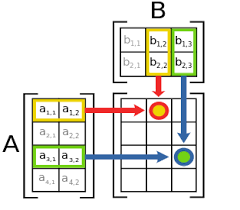
\includegraphics[width=0.3\textwidth]{inc/img/AMulB}
		\caption{ -- Произведение матриц}
		\label{fg:ref2}}
\end{figure}

Операция умножения двух матриц выполнима только в том случае, если число столбцов в первой матрице равно числу строк во второй.

\section{Стандартный алгоритм умножения матриц}
Пусть даны матрицы $A$ (формула \ref{eq:ref1}) размерностью $n \times m$ и $B$ (формула \ref{eq:ref2}) $m \times q$.
\begin{equation}
	B = \left(
	\begin{array}{cccc}
			b_{11} & b_{12} & \ldots & b_{1q} \\
			b_{21} & b_{22} & \ldots & b_{2q} \\
			\vdots & \vdots & \ddots & \vdots \\
			b_{m1} & b_{m2} & \ldots & b_{mq}
		\end{array}
	\right)
	\label{eq:ref2}
\end{equation}

Матрица $C = AB$ будет размерностью $n \times q$.
Тогда каждый элемент матрицы $C$ выражается формулой (\ref{eq:ref3}).
\begin{equation}
	\begin{array}{cc}
		c_{ij} = \sum\limits_{k=1}^m a_{ik}b_{kj} & (i=1,2,\dots n; j=1,2,\dots q)
	\end{array}
	\label{eq:ref3}
\end{equation}

\section{Параллельный алгоритм умножения}

Так как каждый элемент матрицы $C$ вычисляется независимо от других \cite{alg} и матрицы $A$ и $B$ не изменяются, для параллельного вычисления произведения достаточно равным образом распределить вычисление элементов матрицы $C$ между потоками.

В связи с аппаратными ограничениями, производить данные вычисления для каждого элемента результирующей матрицы в отдельности не эффективно. Решением данной проблемы является группировка элементов результирющей матрицы по строкам или столбцам и параллельное вычисление результатов для каждой из данных групп.

\section{Вывод}

Стандартный алгоритм умножения матриц вычисляет элементы результирующей матрицы независимо друг от друга, что позволяет реализовать параллеьный вариант алгоритма.